\chapter{Definizione del Datawarehouse}

L'obiettivo del data warehouse in oggetto è quello di fornire dati relativi
all'utilizzo di veicoli elettrici noleggiati dalla compagnia Helbiz, nel corso
della giornata, al variare delle condizioni meteo e in presenza o assenza di uno
sciopero.
L'architettura scelta è quella a tre livelli, che vede un primo livello costituito
dalle tre sorgenti operative Helbiz, Torino Meteo e Scioperi, un secondo livello
costituito consistente nell'ODS ed un terzo livello costituito dai data mart.

\section{Progettazione concettuale}

Prodotto della fase di progettazione concettuale è il Data Fact Model di figura
\ref{fig:dfm}.

\begin{figure}[H]                                                                                                                                                            
\centering                                                                                                                                                                   
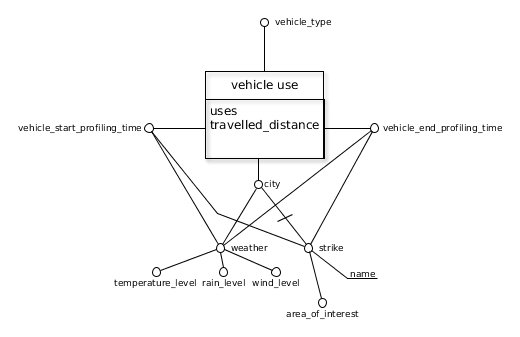
\includegraphics[width=\textwidth]{diagrams/dfm}                                                                                                                                   
\caption{DFM Vehicle use}                                                                                                                                            
\label{fig:dfm}                                                                                                                                                           
\end{figure}

\section{Carico di lavoro}
\begin{table}[h]
\centering
\begin{tabular}{|l|l|}
\hline
\rowcolor[HTML]{3166FF} 
{\color[HTML]{FFFFFF} \textbf{Fatto}} & {\color[HTML]{FFFFFF} \textbf{Interrogazione}}                                  \\ \hline
                                      & Numero di utilizzi durante uno sciopero nelle ore di punta                      \\ \cline{2-2} 
                                      & Numero di utilizzi durante una giornata di pioggia                              \\ \cline{2-2} 
                                      & Numero di utilizzi durante le fasce orarie lavorative                           \\ \cline{2-2} 
                                      & Numero di utilizzi durante le fasce orarie lavorative                           \\ \cline{2-2} 
                                      & Delta del numero di utilizzi tra una giornata di sciopero e una non di sciopero \\ \cline{2-2} 
                                      & Delta del numero di utilizzi tra una giornata di pioggia e una di sole          \\ \cline{2-2} 
\multirow{-7}{*}{Utilizzo veicolo}    & Delta del numero di utilizzi tra una gioranta di pioggia e una di sciopero      \\ \hline
\end{tabular}
\end{table}
\section{Progettazione concettuale}
La progettazione concettuale comporta l’utilizzo dei requisiti identificati nella Sezione xyz
per realizzare uno schema concettuale per il data mart. A tale scopo viene utilizzato il
Dimensional Fact Model (DFM), un modello concettuale creato appositamente per supportare la progettazione di data mart. 
In questa Sezione viene descritta la progettazione del DFM che modella il fatto relativo ad un ascolto.

\section{Progettazione Logica e Fisica}
In questa Sezione viene descritto il processo di trasformazione del DFM, descritto al paragrafo precedente, in modello logico. 
Innanzitutto va specificato che è stata applicata la tecnica ROLAP (Relational On-Line Analytical Processing) che prevede l’utilizzo di un
modello relazionale per la rappresentazione dei dati multidimensionali.
